\section{Data science methodology for breast cancer diagnosis (DSM-BCD)}
A systematic review was conducted in the scientific literature of various methodologies, which although they cover the necessary process for data analysis, they do not generate sufficient value for the solution of a given problem. For this reason, authors such as \cite{Martinez2021} consider that although the data science research community is growing day by day, it is exploring new domains, creating new specialized roles and is making a great research effort to develop advanced analysis, improving models and generating new algorithms supported from the fields of mathematics, statistics and computer science, these skills are not sufficient for application in real projects, since most data-driven projects present organizational and socio-technical problems, such as: a lack of vision and clarity of purpose, a biased emphasis on technical issues, and role ambiguity. And while these problems exist in real-world data science projects, the community has not been too concerned about them and not enough has been written about solutions to address these problems. Given the problems presented by data-driven projects, and the study of various methodologies proposed by several authors, the DSM-BCD (Data science methodology for breast cancer diagnosis) methodology is proposed. This methodology is based on the agile manifesto applied to a context of data-driven results. 

\begin{figure*}
	\centering
	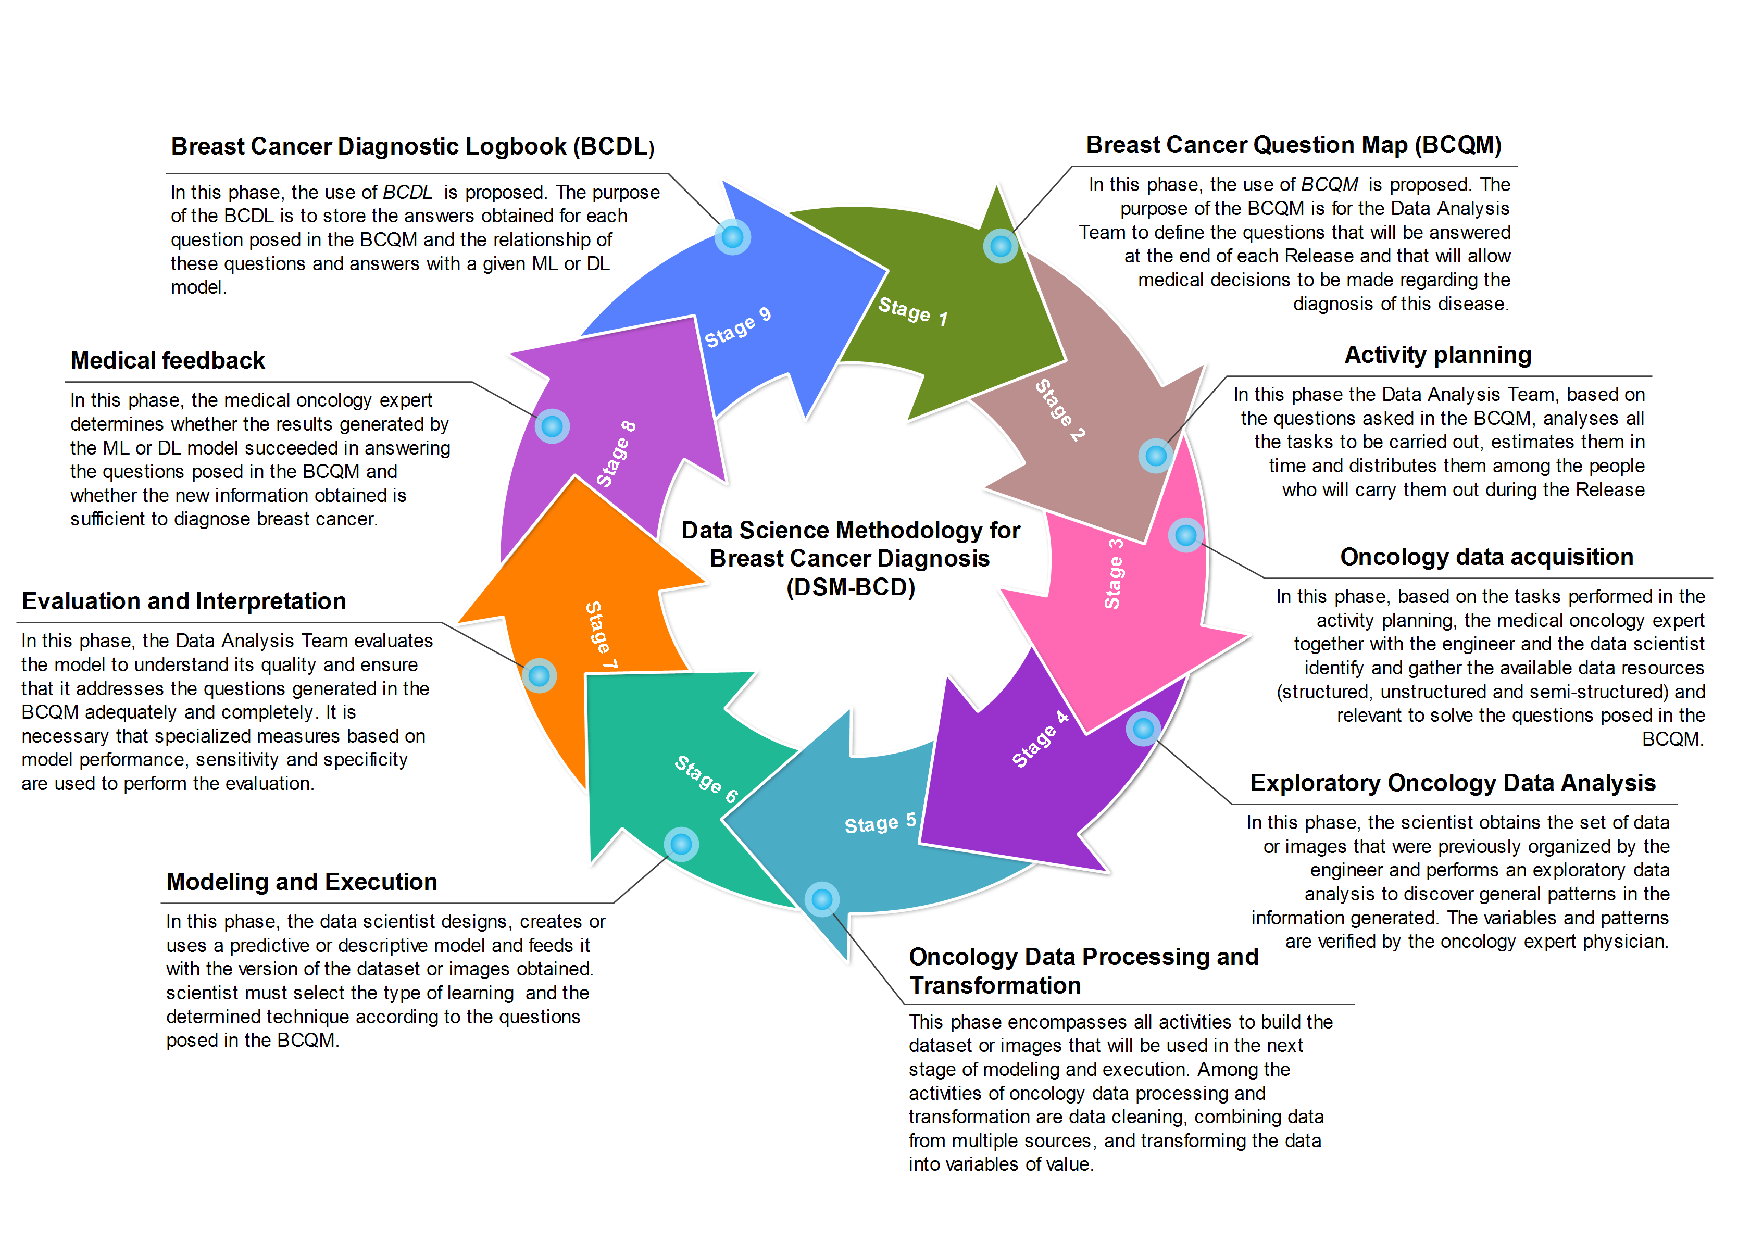
\includegraphics[width=0.9
	\linewidth]{IMAGES/DSM-BCD.pdf}
	\caption{Data science methodology for breast cancer diagnosis (DSM-BCD)}
	\label{DSM-BCD}
\end{figure*}

Given the above, DSM- BCD does not focus on evaluating the accuracy of ML and DL techniques but its main objective is to generate value to the data in the shortest possible time for physicians to diagnose breast cancer in an agile way. To achieve this, DSM-BCD integrates the medical insight and the results obtained by ML and DL techniques in continuous feedback generated in each Release to produce more efficient decision making. In DSM-BCD, a Data Analysis Team is proposed. This team should be headed by the medical oncology expert, at least one data engineer and one data scientist. It is recommended that the team be made up of a maximum of 5 people to facilitate teamwork and internal communication. Figure \ref{DSM-BCD} shows the phases of DSM-BCD. 

\subsection*{Stage 1: Breast Cancer Question Map (BCQM)} 
In this phase, the use of a Breast Cancer Question Map (BCQM) is proposed. The purpose of the \textit{BCQM} is for the \textit{Data Analysis Team} to define the questions that will be answered at the end of each \textit{Release} and that will allow medical decisions to be made regarding the diagnosis of this disease. The BCQM allows you to ask questions related to the types of breast cancer and techniques for breast cancer diagnosis. So that at the end of the time of each Release, which can vary between 1 and 4 weeks, the question will be answered according to the data analysis generated, and the doctor will be able to make a valuable decision. It should be noted that it is possible to have one or more questions related to a technique and a type of breast cancer for each Release, which is why it is possible to find correlations between the characteristic variables of each type of cancer, thus finding hidden patterns in the different data sets. Additionally, the BCQM allows to identify which technique for the diagnosis of breast cancer is related to the question to be solved, which in advance makes it possible to know the type of information (images or data) and the ML or DL algorithm required to solve the problem. Likewise, the BCQM allows to define from the initial phase the type of predictive or descriptive model according to the analytical approach generated by the question posed. Summarizing, the use of BCQM facilitates the understanding of the medical problem and allows to previously identify the technique, the type of information and approach to be used for data analysis. Figure \ref{BCQM} shows the structure of the BCQM.

\begin{figure}[H]
	\centering
	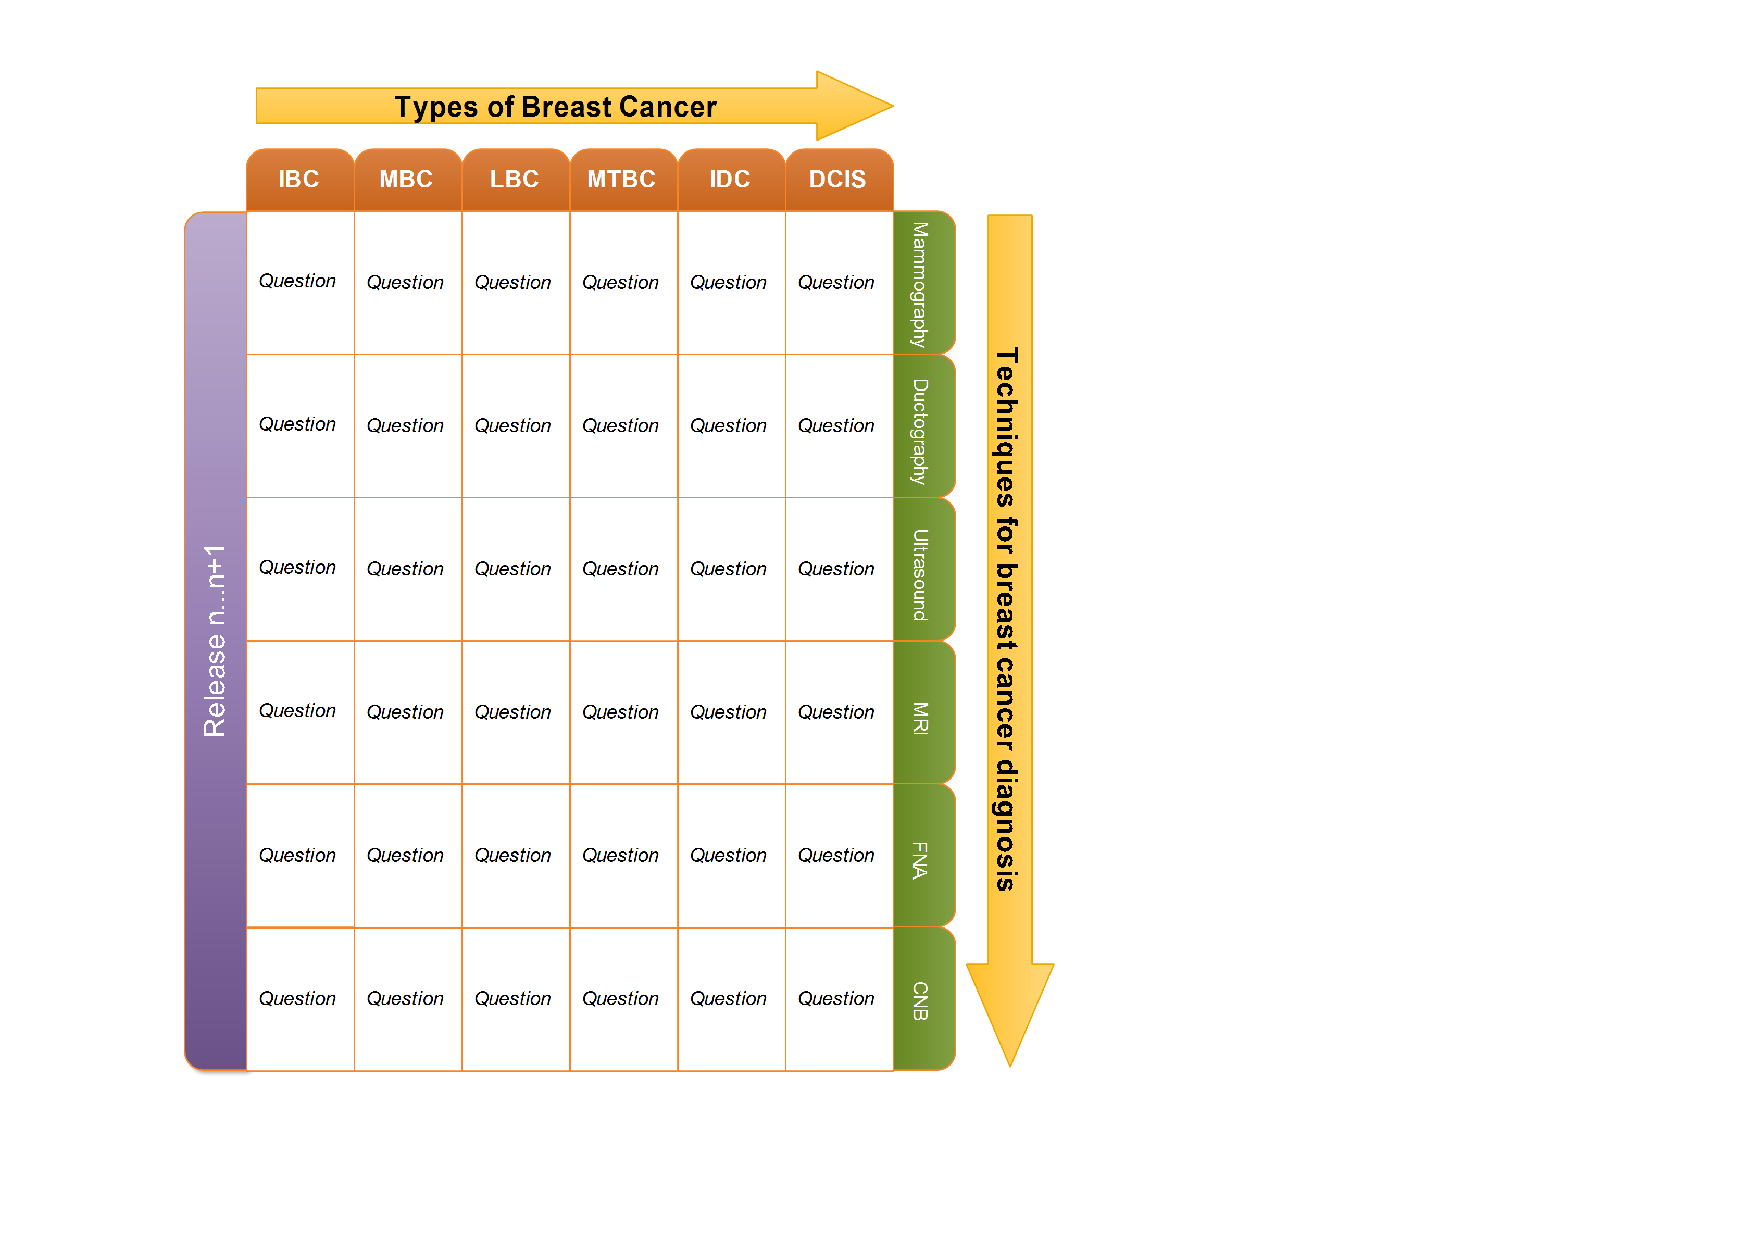
\includegraphics[width=1
	\linewidth]{IMAGES/BCQM.pdf}
	\caption{Map of questions based on inflammatory (IBC), mucinous (MBC), lobular (LBC), mixed tumour (MTBC), invasive ductal carcinoma (IDC) and ductal carcinoma in situ (DCIS) breast cancers.Map of questions based on inflammatory (IBC), mucinous (MBC), lobular (LBC), mixed tumour (MTBC), invasive ductal carcinoma (IDC) and ductal carcinoma in situ (DCIS) breast cancers.}
	\label{BCQM}
\end{figure}

\subsection*{Stage 2: Activity planning }
In this phase the Data Analysis Team, based on the questions asked in the BCQM, analyses all the tasks to be carried out, estimates them in time and distributes them among the people who will carry them out during the Release. Since the BCQM allows us to know in advance the type of breast cancer and the technique for the diagnosis of this disease, the data scientist with the help of the physician can define the data source, which will allow to know the type, quantity and weight of the information. Given the above, it is recommended that the team has at least one data engineer, since he is the one in charge of taking the data and converting it to the data source into meaningful information for the scientist to perform the respective analysis. 

\subsection*{Stage 3: Oncology data acquisition }
In this phase, based on the tasks performed in the activity planning, the medical oncology expert together with the engineer and the data scientist identify and gather the available data resources (structured, unstructured and semi-structured) and relevant to solve the questions posed in the BCQM. It should be noted that in the DSM-BCD methodology it is feasible to have several datasets or images that are related to one type of breast cancer and one diagnostic technique, therefore the Data Analysis Team can have several data scientists answering different questions in the same Release. As a consequence, in the end, multiple answers and a possible correlation between the various oncological variables can be obtained as a result. Also, in this phase the Data Analysis Team must define the necessary data infrastructure according to the amount of information to be processed, which will allow projecting the scalability, scope and distribution of such information. \\ \\

\subsection*{Stage 4: Exploratory Oncology Data Analysis }
In this phase, the scientist obtains the set of data or images that were previously organized by the engineer and performs an exploratory data analysis to discover general patterns in the information generated. It should be noted that in this phase the accompaniment of the medical expert in oncology is of vital importance, since the data or images to be explored by the scientist may contain variables that may or may not have a significant value for the expert, thus helping to determine whether or not the analysis proposed to answer the question is on the right track, so it is possible that several variables are added or eliminated to achieve the expected result. Additionally, it is necessary that the various analyses generated are supported with graphs that are understandable by the entire Data Analysis Team, this for the purpose of providing ideas, and from this phase to find possible correlations between oncological variables.

\subsection*{Stage 5: Oncology Data Processing and Transformation }
This phase encompasses all activities to build the dataset or images that will be used in the next stage of modeling and execution. Among the activities of oncology data processing and transformation are data cleaning, combining data from multiple sources, and transforming the data into variables of value. In this phase, teamwork and continuous communication between the data engineer and data scientist is important to address invalid or missing values, remove duplicates, format, and combine files, tables, and platforms. Additionally, the physician Oncology expert must provide a clearance to proceed with the next phase. This is because the domain expert has a deeper knowledge of the variables or images that are being observed, and if there is unnecessary information for the diagnosis of breast cancer, it is possible to debug that information so that it does not affect the training and subsequent execution of the ML and DL model.

\subsection*{Stage 6: Modeling and Execution}
In this phase, the data scientist designs, creates or uses a predictive or descriptive model and feeds it with the version of the dataset or images obtained in the processing and transformation phase. In this phase, the scientist must select the type of learning (supervised, unsupervised and reinforcement learning) and the determined technique (regression, classification, clustering, CNN, RNN, etc.) according to the questions posed in the BCQM. It is worth mentioning that in this phase the Data Analysis Team must define together with the oncology expert physician the error tolerance allowed in the model, given that the sensitivity of the analysis may vary depending on the type of breast cancer and the diagnostic technique. It is likely that the data scientist will try multiple algorithms with their respective parameters to find the best model for the oncological variables available. It should be noted that it is vitally important that the proposed models do not have problems of over-fitting or under-fitting as this can lead to misleading or insignificant results. Additionally, the data scientist in question together with the Data Analysis Team must define the infrastructure at the server level necessary for training and testing the model according to the amount of information to be processed, with the purpose of generating accurate results in the shortest possible time in order to fulfill the tasks defined in the planning phase of activities and give value to the oncological data once the Release is completed.

\subsection*{Stage 7: Evaluation and Interpretation}
In this phase, the Data Analysis Team evaluates the model to understand its quality and ensure that it addresses the questions generated in the BCQM adequately and completely. It is necessary that specialized measures based on model performance, sensitivity and specificity are used to perform the evaluation. Additionally, the results obtained must be understandable to the oncology physician, ensuring that the results are correctly interpreted and related to breast cancer staging and biomarkers. It is important that the physician and the data scientist adjust the model as needed. Since we are working with sensitive medical data, it is necessary that the final model is applied to a validation set for a final evaluation. In addition, the Data Analysis Team can assign to the model tests of statistical significance as an additional test to check the answer obtained to the generated question. This additional test is essential to justify the implementation of the model. Finally, since the BCQM can ask multiple questions related to different types of breast cancer and diagnostic techniques during the Release, it is necessary for the scientists with the help of the data engineer to join, if possible, the results obtained in a matrix or heat map to identify the correlation coefficient between two or more oncologic variables. This resulting matrix should be analyzed by the medical oncology expert to determine if there is a significant relationship between the different types of breast cancer.
 
\subsection*{Stage 8: Medical feedback}
In this phase, the medical oncology expert determines whether the results generated by the ML or DL model succeeded in answering the questions posed in the BCQM and whether the new information obtained is sufficient to diagnose breast cancer or whether these results generated relevant information to determine the cause or origin of this disease, in short, whether the analyzed data produced added value to the medical domain. In the case that the results obtained did not provide value to the data, the Data Analysis Team will have to decide if it is necessary to re-state the questions or if new data should be acquired to adjust the generated model. In addition, the expert in the company of the data scientist and data engineer, based on their medical acumen, should help decide which strategy is most appropriate to generate meaningful results. Similarly, if the result was satisfactory, the physician should issue an opinion on the level of impact that the information generated by the models had in diagnosing the condition of breast cancer in a given patient and once the information is verified, together with the Data Analysis Team, feed a dataset with the information obtained from the diagnoses generated for each individual. The above with the purpose of improving the performance of existing models and increase their accuracy. Finally, in each Release it must be guaranteed that the diagnosis time is shorter and shorter or that new information is generated that the doctor can use in his daily functions and that helps to determine the origin, relationship or possible treatment of this disease.

\subsection*{Stage 9: Breast Cancer Diagnostic Logbook (BCDL)}
In this phase, the use of a Breast Cancer Diagnostic Logbook (BCDL) is proposed. The purpose of the \textit{BCDL} is to store the answers obtained for each question posed in the BCQM and the relationship of these questions and answers with a given ML or DL model. This log should only be fed when the information obtained generated added value to the medical domain. Its main purpose is to avoid redundancy of information and duplication of questions posed in the BCQM, ensuring that new knowledge related to breast cancer is generated in each Release. It is recommended that the logbook be designed by means of an entity- relationship model (MER) that is made up of entities such as: model, type of breast cancer, diagnostic technique, data set, question and answer. Given the above, it is suggested that the different data sets or images used in the analysis be stored in a cloud-based information hosting service (Amazon Cloud, Google Drive, One Drive, etc.) and that this information be identified with a unique code that facilitates its search when required. Similarly, the different algorithms generated must be stored in a version control system (GitLab, GitHub, Bitbucket, etc.) with their respective operation readme and a unique identification code so that it can be easily consulted by database. Therefore, the use of the BCDL allows to have a detailed traceability of the advances obtained in each Release with respect to the diagnosis of breast cancer, this with the purpose that the Data Analysis Team has a solid starting point to innovate in new ML and DL models through the comparison and continuous improvement of existing models that managed to add value to the different types of oncological data.